\subsection*{СМО с отказами}
\addcontentsline{toc}{subsection}{СМО с отказами}

\textbf{Задание:}\\
На многоканальный телефон (количество каналов N) звонят пользователи с заданной интенсивностью.\\
Если все каналы заняты, клиент получает отказ в обслуживании.\\
Если соединение установлено и есть свободный оператор, принимающий звонки, он общается с клиентом и оформляет заявку.\\
Если все операторы заняты, звонок пользователя отправляется в очередь (FIFO) и ожидает, пока не освободится один из операторов. Если при этом время ожидания превышает заданное значение (T), пользователь прекращает ожидание и кладет трубку.\\
Время общения с оператором случайно, распределено по треугольному закону (параметры задайте самостоятельно).\\
Количество операторов, отвечающих на звонки, определяется расписанием и зависит от дня недели и времени суток.\\
Создайте имитационную модель центра обработки звонков.\\
Определите процентную долю следующих групп звонков:
\begin{enumerate}[topsep=0pt,itemsep=-1ex,partopsep=1ex,parsep=1ex]
	\item Упущенные
	\item Прекратившие ожидание
	\item Обслуженные
\end{enumerate}
Проанализируйте распределение времени ожидания обслуженных звонков. Проанализируйте, как интенсивность звонков, количество каналов и количество операторов повлияют на качество обслуживания.\\

\textbf{Решение:}\\
Для моделирования данной СМО была построена модель в AnyLogic. (Рисунок \ref{fig:vaccination_appointment1})
\begin{figure}[h]
	\centering 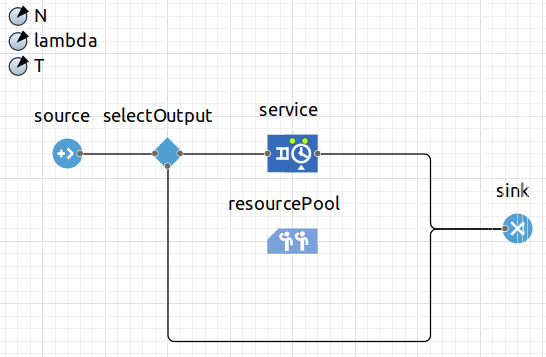
\includegraphics[scale=0.4]{vaccination_appointment1}
	\caption{Схема СМО с отказами}
	\label{fig:vaccination_appointment1}
\end{figure}

\newpage

В качестве интенсивности потока была взята $\lambda = 10$, крайнее время ожидания $T = 5$ и количество каналов  $N = 10$.\\

В данной схеме имеется блок \textit{Source}, в котором с экспоненциальным законом распределения создаются агенты, \textit{SelectOutput}, который отправляет агентов в \textit{Sink}, если количество агентов в блоке \textit{Service} больше 10. Также имеется блок \textit{ResourcePool}, который хранит в себе каналы обслуживания, которые в данной модели выступают как ресурсы.\\

Также в данной модели предусмотрен сбор статистики. (Рисунок \ref{fig:vaccination_appointment2})
\begin{figure}[h]
	\centering 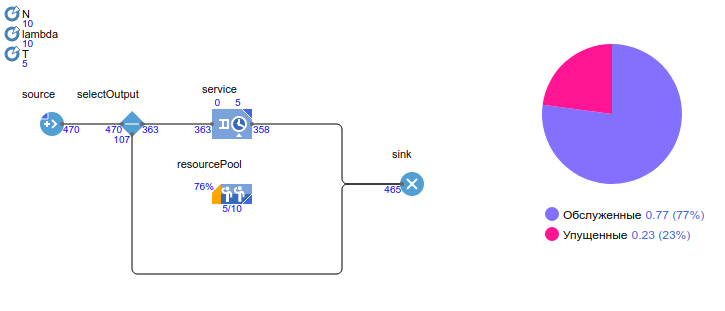
\includegraphics[scale=0.4]{vaccination_appointment2}
	\caption{Сбор статистики}
	\label{fig:vaccination_appointment2}
\end{figure}

Можно видеть, что при данных параметрах обслуженными остались 77\% агентов, оставшиеся остались не обслуженными.\\

Если же варьировать параметры модели, а именно интенсивность входного потока, то можно будет видеть, что с увеличением интенсивности потока -- качество обслуживания понижается, при уменьшении -- наоборот. (Рисунок \ref{fig:vaccination_appointment3})\\
\begin{figure}[h]
	\centering 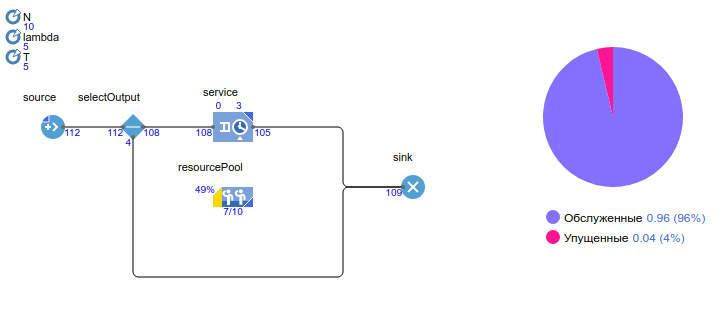
\includegraphics[scale=0.4]{vaccination_appointment3}
	\caption{Уменьшение интенсивности звонков}
	\label{fig:vaccination_appointment3}
\end{figure}

\newpage

Если же варьировать количество каналов обслуживания, то с увеличением числа каналов -- качество обслуживания повышается, а при уменьшении -- наоборот. (Рисунок \ref{fig:vaccination_appointment4})\\
\begin{figure}[h]
	\centering 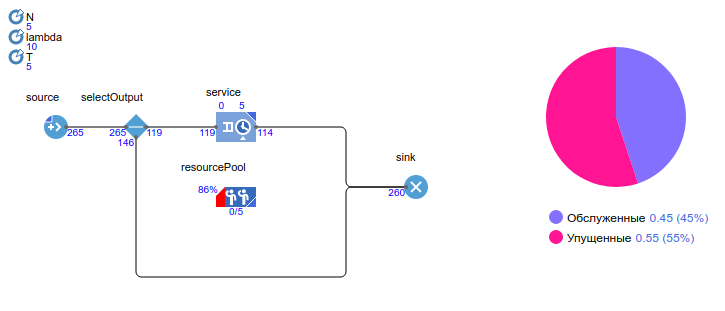
\includegraphics[scale=0.4]{vaccination_appointment4}
	\caption{Уменьшение количества каналов обслуживания}
	\label{fig:vaccination_appointment4}
\end{figure}

Таким образом, была реализована модель центра обработки звонков, было проанализировано влияние факторов на качество её обслуживания.\\

